\subsection{Summing Up} \label{summingUp}
%Goals?
%Test done their job?
%Test in CLS?
To sum up, we have looked at our tests in the perspective of the CLS, meaning how the different tests were decomposed and combinated. We have looked at how this was done both in unit tests and integration tests, while partially covering the effectiveness of these combinators and their structure. We also looked at the tests themselves, how they helped us during development and how they actually help reinforce our code's sturdiness, such that no apparent or obvious bug is present. However, as also covered, we looked at some of the obstacles when creating these tests, both from a synthesis perspective, but also just simply as the tests themselves and how some functions were made difficult to test. We looked over how we worked around some of these obstacles and how some of these were seemingly impossible to work around, at least without changing our code for the tests only. \\
Now that we have covered all these subjects, one may ask, have we been successful in testing and in synthesizing these tests with the CLS? This question has two parts. The first part is the testing itself and how efficiently our code has been tested. The second part is the CLS part, with how well our tests have been decomposed and synthesized, that is, how well does unit testing and integration testing work with the CLS, especially in our case and according to how we implemented them. \\
\\
Let us examine the first part. Have we succeeded in creating tests that efficiently test the correctness of our code? Have we managed to ensure that dead code does not make any apparent or obvious problems with our code? We have already touched upon these questions as we mentioned the benefits of our tests during our development. Here we mentioned how we tested for dead code by using the principles covered in the testing theory section, both in integration tests and the unit tests. So, by using boundary conditions and equivalence partitions, have we successfully tested for the influence of dead code to a satisfactory extent? Well, not entirely. As should be apparent from our section about obstacles in testing, we were not able to cover all the functions. Due to the high coupling between the grains, we had to use mockups for use in unit testing. However, some of the grains could not be fully mocked and as such, we ran into some problems that prevented us from testing certain functions. For instance, the player's TakeDamage function, which is a central part of the player, could not be tested in unit tests, as GetPrimaryKey could not be mocked and as such it gave us an error as the mock tried to access this. On the other hand, with integration tests, we did not rely on mockups and as such did not run into this problem, such that the player's TakeDamage function could successfully be tested in the integration part of the testing. In general, a big part of our troubles with testing stemmed from the use of mockups and how they could not entirely mock grains. However, this was of course not the only reason for our troubles as is apparent from our section on obstacles. \\
In short, as we have been unable to fully test the program, we have only somewhat accomplished testing the correctness of our code. In hindsight, if we had had focus on resolving the high coupling earlier in the process, we might have been able to test better in isolation, that is unit tests. On the other hand, our integration tests, without the mockups, proved easier to implement and we did not run into similar problems when creating these. So, while we would argue that a large part of the program, especially the parts made for variation, have successfully been tested for, some parts of the program was downright impossible to test without interfering with our code and as such, our testing is noncomprehensive and only somewhat satisfactory. \\
\\
Let us now examine the second part. Have we succeeded in synthesizing the tests and how well does our test scale when it comes to the CLS? We have already partially been over this, when we looked at the implementation of unit tests and integration tests in our repository. Because we kept the tests isolated in terms of requirements per test, meaning we only initialized essential parts in the setup, the tests were generally easy to decompose. For instance, as we mentioned, all tests that required the use of boss under player tests, were created specifically in those tests, such that when we decomposed tests, we could do this on a function based level, and thus keeping the ability tests easily separated. Most of the unit tests and integration tests were easily incorporated into our repository and we succesfully connected the tests to the grains, such that creating a specific variation of the game would correctly include the tests specific of that variation as well. As we also went over, most of the tests were also scalable, combinator-wise, in the way that adding new variations of abilities for the boss and player, and specifically tests thereof, could easily be added to the repository, without breaking the current structure of the combinators. \\
\\
The only issue we had with testing in accordance with CLS was the case of the player unit tests. We also mentioned this, how the overlap of the existence of the boss and the player's abilities, made the structure of the player tests combinators somewhat non-trivial and maybe not optimal. If we look at \autoref{testRoarBoss} we can see the case where our variation includes boss and the player ability roar.
\begin{figure}[]
    \centering
    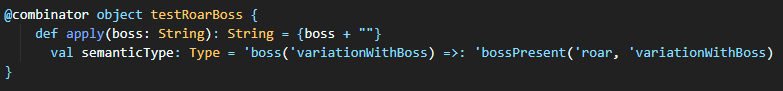
\includegraphics[width=\linewidth]{Materials/TestingDiscussion/testRoarBoss}
    \caption{The "intermediate step" of the player unit test combinator, when we have the variation where the player ability is roar.}
    \label{testRoarBoss}
\end{figure} 
In this specific combinator should be the tests that depend both on roar and boss. As there are no such tests, this combinator is empty. We discussed this earlier, where we came to the conclusion that there would never be a connection between roar and boss directly. This way, isolated, this case seems redundant as we could just have our normal roar tests here, but that would ruin the structure of the player tests. In short, due to one specific test, our entire structure of the combinators have to conform to this, which in all other cases, where the test is not to be included, may seem to be a redundant, but necessary, combinator. This seems somewhat non-scalable as new variations could include new dependencies and thus the entire structure could be changed. However, as stated, we only faced this issue in the player unit tests combinators, while the other combinators were more scalable. This is probably due to the dependencies that these combinators rely on and the nature of these dependencies.\\
\\
All in all, the unit tests and integration tests were remarkably easy to synthesize and as long as you watch out for overlaps that can complicate the synthesis process, this structure of tests makes for great combinators. In short, we would argue that we have succeeded in synthesizing the tests and they scale well as combinators as long as you keep dependencies in check.